\tikzset{every picture/.style={line width=0.75pt}} %set default line width to 0.75pt        

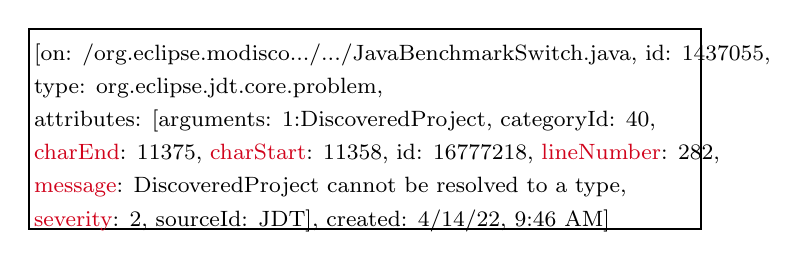
\begin{tikzpicture}[x=0.75pt,y=0.75pt,yscale=-0.7,xscale=0.54]
%uncomment if require: \path (0,300); %set diagram left start at 0, and has height of 300

%Shape: Rectangle [id:dp45731705448754423] 
\draw   (0,1) -- (600,1) -- (600,139) -- (0,139) -- cycle ;

% Text Node
\draw (2,9) node [anchor=north west][inner sep=0.75pt]   [align=left] {{\footnotesize [on: /org.eclipse.modisco.../.../JavaBenchmarkSwitch.java, id: 1437055, }\\{\footnotesize type: org.eclipse.jdt.core.problem, }\\{\footnotesize attributes: [arguments: 1:DiscoveredProject, categoryId: 40, }\\{\footnotesize \textcolor[rgb]{0.82,0.01,0.11}{charEnd}: 11375, \textcolor[rgb]{0.82,0.01,0.11}{charStart}: 11358, id: 16777218, \textcolor[rgb]{0.82,0.01,0.11}{lineNumber}\textcolor[rgb]{0,0,0}{:} 282,}\\{\footnotesize  \textcolor[rgb]{0.82,0.01,0.11}{message}: DiscoveredProject cannot be resolved to a type,}\\{\footnotesize  \textcolor[rgb]{0.82,0.01,0.11}{severity}: 2, sourceId: JDT], created: 4/14/22, 9:46 AM]}};


\end{tikzpicture}
